\chapter{重症急性胰腺炎}

\section{前沿学术综述}

重症急性胰腺炎的全病程大体可以分为3期
\protect\hyperlink{text00021.htmlux5cux23ch1-20}{\textsuperscript{{[}1{]}}}
(并非所有患者都有3期病程)------①急性反应期:自发病至2周左右,以全身炎症反应为特征,主要矛盾是全身炎症反应综合征(systemic
inflammatory response
syndrome,SIRS),常伴有休克、ARDS、急性肾衰竭和胰性脑病等主要并发症;②全身感染期:2周至2个月左右,以胰腺或胰周坏死感染为特征,局部的感染极易发展为脓毒症(sepsis),甚至多器官功能障碍;或双重感染为其主要临床表现;③残余感染期:时间为2~3个月以后,主要临床表现为全身营养不良,存在后腹膜或腹腔内残腔,常常由于引流不畅,导致窦道经久不愈,伴有消化道瘘。如果重症急性胰腺炎的局部炎症得到有效控制,局部坏死组织没有感染,病程可不进入感染期,而在2周左右直接转入恢复期。

\subsubsection{重症急性胰腺炎严重程度评估}

重症急性胰腺炎病情的变化迅速,预后凶险,单凭临床经验有时难以正确估计,严重度的评估有利于了解病情,以指导临床治疗,因而具有十分重要的临床意义。急性胰腺炎严重度估计包括3个方面:全身评分系统、局部估计以及多器官功能不全评分系统,有学者曾经研究过血清标记物,希望用C反应蛋白、中性粒细胞弹力蛋白酶和胰蛋白酶激活肽等单项生化指标评估严重度,但目前都无法作为临床应用的可靠指标。

(1)全身评分系统

Ranson评分 20世纪70年代初,Ranson
\protect\hyperlink{text00021.htmlux5cux23ch2-20}{\textsuperscript{{[}2{]}}}
提出的评分被认为是急性胰腺炎严重度估计指标的里程碑。当时采用腹腔灌洗治疗胰腺炎,然而哪些胰腺炎患者需要灌洗治疗呢?Ranson评分就在此背景条件下产生,该评分系统包括入院时的5项临床指标和入院48小时的6项临床指标,合计11分。当评分在3分以上时,即为重症胰腺炎,需要做灌洗治疗。同时发现胰腺炎患者的Ranson评分与病死率有明显的关系:3分以下的病死率为0.9%,3~4分为16%,5~6分为40%,6分以上为100%。

Imrie评分 为在Ranson评分的基础上改良而成。入院48小时评分包括白细胞计数、血糖、血尿素氮、动脉氧分压、血钙、肝功能等8项指标,其特点是包含了血浆白蛋白浓度。该评分在英国应用较广。Ranson评分和Imrie评分根据都是患者入院24或48小时内的病情,不能动态估计严重度,而且评分未包括患者以往的身体状况(例如对于一个原有门静脉高压的患者受到急性胰腺炎的打击,其预后与正常人发生急性胰腺炎有明显的差别)。

APACHEⅡ评分 1985年,Knaus对最初提出的APACHE评分进行修改,称为APACHEⅡ评分。该评分采用12个急性生理指数,结合年龄因素、慢性健康评分和Glasgow昏迷评分,共15项。由于APACHEⅡ评分也能对急性胰腺炎的严重度进行临床评估,在1992年美国亚特兰大举行的急性胰腺炎国际会议上
\protect\hyperlink{text00021.htmlux5cux23ch3-20}{\textsuperscript{{[}3{]}}}
,将Ranson评分在3分或3分以上,或APACHEⅡ评分在8分或8分以上规定为重症胰腺炎。会议指出,Ranson评分在发病48小时后不能应用(此处发病48小时等同于入院48小时,是假设患者发病后立即入院),而APACHEⅡ评分能在急性胰腺炎病程的任何时间内应用。会议还指出,在患者入院以及采用任何治疗方法时进行严重度评分,以便于不同医院和部门之间、国内和国际间比较临床资料,是学术交流的必备临床资料。

(2)局部严重度估计 所有的全身评分系统都仅针对疾病严重度,不具备对急性胰腺炎的特异性,因而研究人员又从胰腺病变的局部来研究对急性胰腺炎严重度的估计。

手术切除胰腺坏死组织称重 Beger采用称重手术切除胰腺坏死组织的方法估计胰腺坏死的程度,坏死面积3cm×5cm,切除的坏死组织少于50g时,胰腺坏死为30%;坏死面积5cm×8cm,切除的坏死组织少于120g,胰腺坏死为50%;大面积暗红色坏死组织,仅残留少许有生命力的黄色组织,坏死组织的重量超过120g,为次全胰坏死;无健康组织存在,坏死组织超过190g,为全胰腺坏死。但该方法只适用于手术患者,而且不能动态观察病情的变化。

根据腹腔渗液的量和颜色 Mcmahon根据腹腔渗液的量和颜色来表示急性胰腺炎病变的严重度。凡符合下列3个标准中任何1项即为重症胰腺炎:①抽吸游离腹腔渗液的量超过10ml(5年后Mcmahon将抽出的液体量改为20ml);②腹腔渗液为深紫红色,无论其量的多少;③用1L生理盐水灌洗腹腔后,仍抽吸到较深颜色的液体。该判断标准的缺点是只能在入院时采用,不能动态观察病情,对颜色的判断有主观差异,只能判别轻重型,因此目前已很少应用。

胰腺称重和抽吸腹水的观察都不是理想的估计急性胰腺炎严重度的方法。

CT评分 20世纪80年代中期,CT的临床应用已相当成熟,动态的增强CT扫描已经是临床诊断胰腺炎有无坏死和坏死程度的金标准,Balthazar
\protect\hyperlink{text00021.htmlux5cux23ch4-20}{\textsuperscript{{[}4{]}}}
的评分系统包括了胰腺和胰外的病变,定量较为准确,评分方法简单易掌握。由于CT检查是非创伤性的,可以动态观察、多次检查,观察胰腺病变是恶化还是改善,所以在局部估计的方法中具有独特的优点。在众多的CT检查评分中,Balthazar的CT评分系统在全世界范围影响较广,已广泛地应用于科研和临床工作中。

(3)多器官功能障碍的评价 全身评分系统和局部估计对急性胰腺炎严重度的评分和预测,不能代替对伴发多器官功能障碍综合征(MODS)及其病死率的评估和预测,APACHEⅡ评分中的慢性健康状况虽然涉及器官系统功能衰竭或免疫功能障碍,急性生理指标中包括部分脏器功能指标,如血肌酐、心率、Glasgow昏迷评分等,但也未能代表完整的器官功能。唯有多器官功能障碍综合征的评分系统能全面估测器官功能的变化。关于器官功能衰竭的评分系统非常多,如急性器官功能衰竭(acuteorgansystemfailure,ADSF)评分、多器官功能衰竭评分等都是针对终末期患者所制定,不适合早期重症胰腺炎的器官功能评估。重症胰腺炎的患者往往在发生多器官功能衰竭前先出现多器官功能障碍综合征,因此目前多采用Marshall
\protect\hyperlink{text00021.htmlux5cux23ch5-20}{\textsuperscript{{[}5{]}}}
的多器官功能障碍综合征评分系统评估器官功能。

由于重症胰腺炎患者既存在局部病变,又有全身病变和(或)伴器官功能损伤,重症急性胰腺炎的评估应结合全身、局部和多器官功能评估,目前通常分别采用APACHEⅡ评分、Balthazar的CT评分和Marshall的评分系统,这样可以获得良好的病情判断和预后评估。

(4)急性胰腺炎预后预测评分(the pancreatitis outcome prediction
score,POP评分) 该评分指标包括年龄、平均动脉压、氧合指数、动脉血pH值、血清尿素氮和血钙浓度。2007年提出来,但至今没有被广泛采用。

\subsubsection{重症急性胰腺炎早期病理生理特点}

(1)SIRS 重症急性胰腺炎通常是以局部非感染性炎症开始,在数分钟到数小时内就可能出现全身炎症反应,并逐渐影响全身多个器官的功能。炎症反应期从病程开始到7~10天临床表现为发热、心动过速、白细胞增多等症状,甚至发展为多器官功能障碍综合征。病情虽然危重,但在现代重症医学科内可争取较高的生存率。

(2)血流动力学改变 急性重症胰腺炎时的循环功能改变以血液分布异常为特点
\protect\hyperlink{text00021.htmlux5cux23ch6-20}{\textsuperscript{{[}6{]}}}
,循环容量不仅因为局部渗出、腹水、呕吐等原因而绝对不足,而且,由于血管的异常扩张导致相对不足。可以表现为心动过速、少尿、休克等。这时应首先根据临床表现密切注意循环容量的改变,应及时进行血流动力学监测,可以有效地指导早期治疗中的容量复苏及整个治疗过程中的精细容量调节。

急性重症胰腺炎时心脏可出现明显的损伤,重症胰腺炎可见骤然死亡病例,尸检时发现心脏有明显的损害,如心肌梗死、心内膜炎或传导系统损害。急性胰腺炎对心血管的损害,原因尚不甚明了。现今认为系胰酶进入血循环,引起冠状动脉痉挛,胰蛋白酶及多肽类物质直接损害心肌;胰腺炎性渗出液积存于腹膜后,刺激腹腔神经丛,反射性广泛性血管痉挛等因素所导致。有人认为系胰腺内含有心肌抑制因子,其根据是将胰腺做成匀浆注入动脉体内可抑制心肌用氧。亦有人提出在急性胰腺炎时释放某种物质,使心肌传导系统兴奋而致心律紊乱,以至心室纤维颤动。

重症急性胰腺炎和创伤对心肌的影响不同。创伤后机体的即刻反应是心肌收缩力增强。已经证实在创伤后的即刻阶段心室射血分数大于恢复期。重症急性胰腺炎往往与感染的情况相似,在重症急性胰腺炎情况下,心室射血分数明显下降。尽管内源性儿茶酚胺增多,但心肌收缩力并不增加,提示心肌β受体功能减弱。与创伤相比,重症急性胰腺炎早期需要更高的前负荷。重症急性胰腺炎患者经过早期容量复苏后,体循环阻力往往是降低的。这是由于炎性介质的作用使周围血管异常扩张,血液重新分布所致。这是重症急性胰腺炎出现顽固性低血压的主要原因。

(3)呼吸功能变化 重症急性胰腺炎是ARDS的强烈诱因,患者在早期所表现的过度通气往往被忽视。但随之而来的常是ARDS的典型临床过程。随着病程的延续,可在ARDS基础上出现肺部感染,甚至成为主要的感染源,对重症胰腺炎时呼吸系统的监测主要是炎症反应期对ARDS发生发展的监测和感染期对ARDS继续恶化及合并肺部感染的监测。在重症急性胰腺炎初期,患者可表现为轻度呼吸频率加快,多无明显呼吸困难,听诊两肺多清晰,无啰音。血气检查仅表现为过度通气,动脉二氧化碳分压下降,动脉氧分压在正常范围。这段时间可维持3~5天,如果观察不仔细则极易漏诊。之后,低碳酸血症逐渐加重并发生低氧血症,提高吸入氧浓度,动脉氧分压不能提高到相应水平,呼吸困难逐渐加重,可出现紫绀,听诊双肺啰音开始增多,胸部X线片表现为双肺弥漫性、对称性密度增高,以间质水肿为主。有时由于肺部合并感染,可使胸部X线表现不典型。此时已经表现出明显的ARDS,需用机械通气方能维持动脉氧分压在正常范围。如果病情进一步恶化,肺部感染加重,可出现大片肺实变、肺不张,低氧血症与高碳酸血症并存,患者出现昏迷、混合性酸中毒等。

对于重症急性胰腺炎合并ARDS的患者可以采取呼吸动力学监测。呼吸动力学监测是根据物理学的原理,采用物理学的参数对呼吸器官的功能进行监测,其监测指标主要包括容积、压力、阻力、顺应性和呼吸做功等项指标。目前,临床上已经可以同步、连续地测量上述有关指标的变化。如描记压力容量曲线不仅可以及时了解病情的演进,还可以反馈性指导临床治疗,目前较多用于对机械通气过程的监测。这些指标与血液动力学指标相结合会给治疗带来更大的帮助。

\subsubsection{重症急性胰腺炎的临床表现}

急性胰腺炎的病理变化的不同阶段,其全身反应亦不一样。同时由于发病时间、机体的状况亦可表现有较大的差异。概括的表现是:轻型胰腺炎主要症状为腹痛、恶心、呕吐、发热,而重症急性胰腺炎的症状除上述情况外,又因胰腺有出血、坏死和自溶,还可出现休克、高热、黄疸、腹胀以至肠麻痹、腹膜刺激征以及皮下出现淤血斑等。

(1)腹痛 为最早出现的症状,往往在暴饮暴食或极度疲劳之后发生,多为突然发作,位于上腹正中或偏左。疼痛为持续性进行性加重、似刀割样。疼痛向背部、胁肋部放射。剧烈的腹痛多系胰腺水肿或炎性渗出压迫、刺激腹腔神经丛引起。若为出血坏死性胰腺炎,发病后短暂时间内即为全腹痛,急剧腹胀,有向腹内打气感,同时很快即出现轻重不等的休克。

(2)恶心、呕吐 为炎性因子刺激迷走神经的表现,发作频繁,起初呕吐物为进入食物或胆汁样物,在病情进行性加重(或发展为出血坏死性胰腺炎)时,患者很快即进入肠麻痹,则吐出物为粪样。

(3)黄疸 急性水肿型胰腺炎出现得较少,约占1/4。而在急性出血性胰腺炎则出现得较多。黄疸的出现多由于:①同时存在胆管结石嵌顿;②胆总管开口水肿、痉挛;③肿大的胰头压迫胆总管下端;④因病情重笃、腹腔严重感染而造成肝功能损害。

(4)脱水 急性胰腺炎的脱水主要因肠麻痹、呕吐所致,这是轻型的原因。而重型胰腺炎在短短的时间内即可出现严重的脱水及电解质紊乱,主要原因是因后腹膜炎症刺激,可有数千毫升液体渗入后腹膜间隙,似无形丢失。出血坏死型胰腺炎,发病后数小时至数十小时即可呈现严重的脱水现象,无尿或少尿。

由于胰腺大量炎性渗出,以至胰腺的坏死和局限性脓肿等,可出现不同程度的体温升高。若为轻型胰腺炎一般体温在39℃以内,3~5天即可下降;重型胰腺炎则体温常在39~40℃,常出现谵妄,持续数周不退,并常常提示合并脓毒症。

少数出血坏死性胰腺炎,胰液以至坏死溶解的组织沿组织间隙可达到皮下,并溶解皮下脂肪而使毛细血管破裂出血,导致局部皮肤呈青紫色,有的可融成大片状,可在腰部前下腹壁出现(Grey-Turner征),亦可在脐周出现(Cullen征)。

(5)腹腔高压 腹胀和腹膜后渗液可导致腹腔高压,严重者可导致腹腔间隔室综合征。腹腔高压可带来一系列的病理生理变化,包括高气道阻力、低氧血症及高碳酸血症;回心血量及心输出量的减少、低血压;少尿、无尿;颅内压明显升高;器官灌注压明显降低、肝动脉血流减少、肠道灌注下降等。

胰腺的位置深在腹膜后,一般的轻型水肿型胰腺炎在上腹部深处有压痛,少数前腹壁有明显压痛,而重症急性胰腺炎,由于其大量的胰腺溶解、坏死,出血则前、后腹膜均被累及,全腹出现肌紧张、压痛,全腹胀气,并可有大量炎性腹水,可出现移动性浊音,肠鸣音消失,并且出现麻痹性肠梗阻。

由于渗出液的炎性刺激,可出现胸腔反应性胸水。临床以左侧多见,可引起同侧的肺不张,出现呼吸困难。

大量的坏死组织积聚于小网膜囊内,在上腹可以看到一隆起性包块,触之有压痛,往往包块的边界不清。少数患者腹部的压痛等体征不明显,但仍然有高烧、白细胞增高以至经常性出现“部分性肠梗阻”的表现,从而在腹腔或盆腔形成局限性脓肿,此时应做B超检查和肛门指检。

\subsubsection{重症急性胰腺炎的治疗}

目前国内外趋于一致的策略概括为:在重症急性胰腺炎的早期,采取以脏器功能支持为中心的非手术治疗,无菌性坏死尽量采取非手术治疗,出现坏死感染后采用手术治疗
\protect\hyperlink{text00021.htmlux5cux23ch1-20}{\textsuperscript{{[}1{]}}}
。

(1)非手术治疗 重症急性胰腺炎起病初期应在重症医学科内监护治疗,原则是补充体液、维持水电解质平衡、能量支持、防止局部及全身并发症的出现。监测内容包括生命体征、动脉血氧饱和度、尿量/小时、水电解质、肌肝、尿素氮、血常规、动脉血气、X线胸片。早期处理包括,液体复苏、氧疗、禁食、止痛,H\textsubscript{2}
受体拮抗剂、胃肠减压等,重点在于器官功能的维护;特殊治疗包括抑酶制剂、抗胰腺分泌药、血小板活化因子拮抗剂(如Leipafant)、预防性使用抗生素(在抗生素使用上,推荐有胰腺坏死者使用碳青霉烯类)。早期防治ARDS、急性肾衰竭、休克、DIC、代谢性脑病等并发症。

除此之外,目前世界各地在重症急性胰腺炎的非手术治疗方面都进行了多项探索,包括持续血液滤过
\protect\hyperlink{text00021.htmlux5cux23ch7-20}{\textsuperscript{{[}7{]}}}
\textsuperscript{,}
\protect\hyperlink{text00021.htmlux5cux23ch8-20}{\textsuperscript{{[}8{]}}}
、腹腔灌洗等,但其作用尚待进一步研究证实。

(2)微创治疗 当前重症急性胰腺炎的微创治疗方法包括辅助治疗的微创化和针对重症急性胰腺炎局部并发症的微创治疗,前者包括胆道引流微创化等,后者包括假性囊肿穿刺引流、胰周脓肿穿刺引流和胰腺坏死感染的微创治疗等,近年来最大的热点和进展在于胰腺坏死感染的微创治疗。

重症急性胰腺炎微创治疗实践开始较早,现大多已成熟,并广泛应用于临床。主要包括:①胆道引流,经皮胆囊穿刺置管引流、内镜下鼻胆管置管引流和内镜下鼻胆管置管引流加乳头肌切开术,目前这些技术可以替代绝大多数的急诊开腹胆道引流;②空肠喂养管的放置,目前可以在内镜、X线或无线电等引导下放置鼻空肠管,也可以在内镜引导下经皮穿刺放置空肠喂养管,这些技术同样可以替代绝大多数的开腹空肠造口术;③腹腔积液的引流,B超或CT引导下经皮穿刺引流腹腔积液,引流效果通常较好。然而,有学者不主张积极穿刺引流,主要是考虑其有自行吸收的机会及穿刺引流潜在的污染可能,也有学者主张应积极引流,因为积液较多可造成腹腔高压、并有致炎作用及潜在的感染风险,但目前仍缺乏更多的循证医学依据。

对于重症急性胰腺炎合并胰周脓肿的微创治疗,主要采用超声或CT引导下经皮穿刺置管引流和内镜引流,临床效果较为肯定,大部分指南都予以推荐。

对于重症急性胰腺炎合并胰腺坏死感染的微创治疗,既往认为感染的胰腺坏死组织是手术引流的绝对适应证,但自1998年Freeny
PC等首次在CT引导下经皮穿刺置管引流用于治疗感染的胰腺坏死组织以来,微创技术目前已广泛应用于治疗感染的胰腺坏死组织。近年来聚焦的热点在于经皮穿刺置管引流适应证的选择、内镜技术的发展以及各种引流技术的有效结合。我们的实践表明,感染的胰腺坏死组织CT密度平均值和CT范围值均为经皮穿刺置管引流治疗胰腺坏死组织感染的影响因素,其值越大,失败的风险性越高,不适合选择经皮穿刺置管引流;反之则建议首先选择经皮穿刺置管引流。与此同时,内镜技术的发展也明显提高了感染的胰腺坏死组织的引流效果。Seifert
H等采用内镜下经胃腔直接引流感染的胰腺坏死组织,Belle
S等则在内镜下通过置入自身扩张的金属支架引流坏死组织。近年来更重要的进展在于将穿刺引流技术和内镜技术有效结合引流感染的坏死组织。Raraty
MG等也同样报道了将穿刺引流技术和内镜技术有效结合引流感染的坏死组织的临床效果。

南京军区南京总医院从2010年开始发展了经皮穿刺持续负压冲洗引流结合内镜辅助坏死组织清除术,获得较好的疗效。从2008年至今,南京军区南京总医院重症急性胰腺炎合并坏死感染病人开腹手术的比例从2007年的100%下降到了2011年的21%,越来越多的重症急性胰腺炎病人避免了开腹手术。

(3)手术治疗 包括两种:①胰腺坏死组织清除术,采用钝性或用吸引法将坏死组织清除,在胰床、小网膜囊、双侧结肠后等部位放置引流,持续性局部灌洗引流。从临床资料来看,胰腺坏死组织清除术的手术有较为合理、简便易行、损伤性小、并发症少、病死率低等优越性。②腹部开放填塞,其方法是打开小网膜囊后充分游离胰腺,并清除坏死组织,于暴露的横结肠系膜、大血管上、胃后壁上盖以非粘性多孔纱布保护,再用生理盐水纱布堵塞。腹壁可以疏松缝合;亦可采用“三明治式”技术,将聚丙烯网片覆盖于暴露的内脏或网膜上,再缝于切口双侧筋膜边缘,外覆透明手术粘贴巾,吸引管置于两层之间;每次换药时去掉粘贴巾,切开网膜片入腹,手术结束时缝合网片,外覆透明粘贴巾,又恢复了“三明治式”结构。以上两种方法各有其利弊。亦有人提出若干种关腹方法,原则是要简单,便于再次换药,防止混合感染。

\section{临床问题}

\subsection{临床特征与诊断}

\subsubsection{Ranson评分和APACHEⅡ评分对评价急性胰腺炎有何利弊?}

Ranson评分是急性胰腺炎常用的评分系统,但要48小时后才能建立,一些指标受治疗等因素影响,不能重复应用。主要是用于酒精性胰腺炎,对胆源性的敏感性和特异性不佳。

APACHEⅡ评分的优点是不但有急性指标和年龄参数,还有慢性健康评分,其次是不受入院后的时间限制,可反复评估严重度,能在急性胰腺炎病程的任何时间内应用。评分降低表示病情好转,评分增加表示病情恶化,评分越高,病情越严重,因而达到动态观察、监测疾病过程的目的。但该评分非急性胰腺炎的特异评分。

\subsubsection{如何对重症急性胰腺炎患者进行CT评分?}

表\ref{tab15-1}对照CT根据胰腺炎症分级和胰腺坏死范围的两方面进行评分,所得积分评定3级严重度:Ⅰ级,0~3分;Ⅱ级,4~6分;Ⅲ级,7~10分。有研究表明,低于2分者无死亡,7~10分的病死率为17%,高于7分可以做手术治疗;A、B级无并发症,C、D、E级时脓肿发生率为34.6%,D级病死率为83%,E级病死率为17.4%。提示CT评分对急性重症胰腺炎的预后和并发症的发生具有较好的预测价值。

\begin{table}[htbp]
\centering
\caption{Balthazar的CT评分系统}
\label{tab15-1}
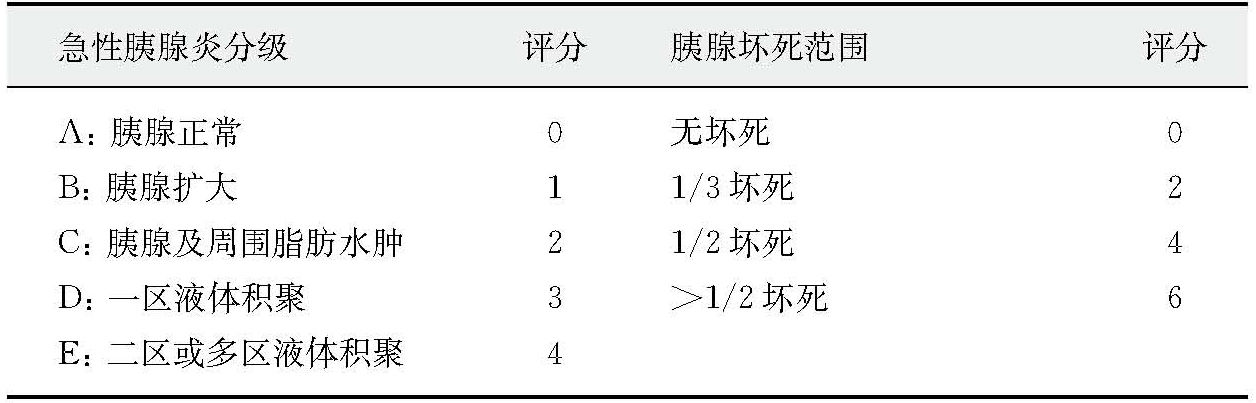
\includegraphics{./images/Image00114.jpg}
\end{table}

\subsubsection{如何对重症急性胰腺炎患者进行多脏器功能障碍评分?}

多器官功能障碍(MODS)评分系统用6个器官系统的简单生理指标来反映器官功能(表\ref{tab15-2})\footnote{*氧合指数的计算,不考虑是否应用呼吸机和呼气末正压水平;血清肌酐不考虑是否接受血液透析治疗;压力调整的心率=心率×(中心静脉压/平均动脉压)。},这些器官是肺、肾、肝、心血管、血液学和神经系统。肺、肾、肝功能分别用吸入氧浓度和动脉血氧浓度的比值、血肌酐浓度、血胆红素浓度来表示,心血管系统用心率、中心静脉压与平均动脉压的比值表示,血小板浓度表示血液系统功能,Glasgow昏迷评分评价神经系统功能。每个器官系统分为5个等级,分别为0、1、2、3、4分,正常为0分,异常有4个等级,器官系统功能异常的最高评分为24分。MODS评分系统可正确反映重症医学科危重患者、包括重症胰腺炎患者的病死率,反映出器官功能的改善或恶化,以指导临床治疗措施。评分在9~12分的患者病死率为25%;13~16分和17~20分的病死率分别为50%、75%;评分高于20分的病死率为100%。

\begin{table}[htbp]
\centering
\caption{MODS评分系统\textsuperscript{*}}
\label{tab15-2}
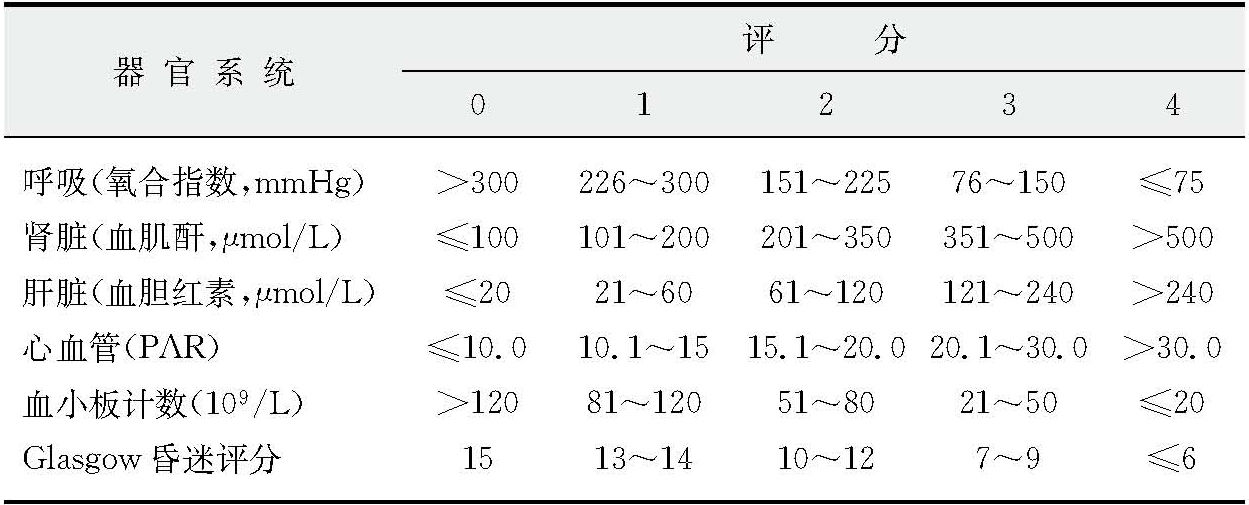
\includegraphics{./images/Image00115.jpg}
\end{table}



\subsection{治疗原则}

\subsubsection{胰腺炎患者收入重症医学科治疗的指征是什么?}

根据重症急性胰腺炎患者的管理指南(critical care medicine
2004,32:2524-2536)建议,重症急性胰腺炎应按照常规的入住标准收住重症医学科。另外,对于老年、肥胖、需要持续容量复苏和有实质胰腺坏死的患者,因其病情迅速恶化的风险高,必须考虑在过渡病房或重症医学科治疗(level5,D级)。

建议(1):危重的急性胰腺炎患者由重症医学科专家领导的多专业小组来治疗,小组人员含消化内镜、内镜下逆行胰胆管造影术技能的内科医师、外科医师和介入放射科医师组成。

建议(2):不管胰腺炎患者在什么病房治疗,都须严密观察病情。临床监测生命体征,评价容量(物理检查、尿量和酸碱情况)、肺功能(如低氧血症)和肾脏功能等。

建议(3):疾病特异评分和病情严重度评分,有助于判断出现并发症风险的高低,但不能替代连续的临床评估(level5,D级)。

\subsubsection{重症急性胰腺炎患者早期的液体复苏有哪些特殊性?}

充分的组织氧供是重症急性胰腺炎患者多器官功能障碍综合征(MODS)防治的重要环节。在治疗中,要注意早期液体复苏、维护组织供氧、防治休克和MODS。在重症急性胰腺炎早期,胰腺坏死出血,造成有效容量快速丢失,同时毛细血管通透性明显增加,造成“毛细血管渗漏”,大量液体自血管内向组织间隙转移,有效循环血量急剧减少,组织水肿。不充足的液体复苏往往导致早期器官功能障碍,及时纠正低血容量和低氧血症有助于维护氧输送,在中心静脉压或肺动脉嵌顿压指导下进行扩容治疗,适当增加胶体的补充,避免或减轻因组织低灌注所致脏器功能的损害。初期液体复苏达到末梢循环恢复,尿量充足,呼吸、心率和血压平稳后,要继续密切监测这些参数的变化。在重症急性胰腺炎早期,血管内皮通透性增加所致间质水肿、毛细血管渗漏等,会给液体复苏增加难度。因此,重症急性胰腺炎的液体复苏治疗往往有以下特殊注意事项:

(1)早期液体需求量大,病情越重患者液体缺失越多,补液量就越大。

(2)由于患者往往存在腹腔高压,导致中心静脉压和(或)肺动脉嵌顿压测量数值偏高,不认识到这一点,往往因这些测量数值误导治疗,中心静脉压和肺动脉嵌顿压则逐渐升高,已不能准确反映血管内容积状况。在这种情况下,如果根据中心静脉压和肺动脉嵌顿压的升高及心输出量的下降而快速利尿,会加重病情。此时,左室舒张末期容积指数是反映血管内容积状态的最佳指标,如不能监测,应结合患者的腹腔压力、尿量、心率、血压等综合判断。动态中心静脉压或肺动脉嵌顿压测量数值往往更有意义,必要时做补液试验观察中心静脉压或肺动脉嵌顿压的变化,对临床判断更有帮助。

(3)补充过多晶体液往往加重组织水肿、肺水肿,加重低氧血症、肠道水肿,加重腹腔高压和肠道功能障碍。因此,在液体复苏早期可以晶体为主,但后期应增加胶体比例,达到1∶1~2。

\subsubsection{重症急性胰腺炎患者腹腔高压会造成哪些不良影响?}

腹内高压在一定程度上反映重症急性胰腺炎患者的病情严重程度,因此在监护治疗中,要注意腹内压的监测。一方面,腹内压的进行性升高预示腹部情况未得到有效控制;另一方面,腹内高压还会引起或加重脏器功能障碍,最常受累的是心、肺和肾脏,还可以引起肝、肠道和大脑的功能障碍或紊乱。腹腔高压不利的病理生理学影响如下。

(1)胃肠道 是对腹腔内压力升高最敏感、受腹内高压及腹腔间隔室综合征影响最早的器官。当腹腔内压力达10mmHg时,小肠黏膜血流灌注减少17%;腹腔内压力达20mmHg时,血流灌注减少36%;腹腔内压力达40mmHg时,血流灌注减少67%,而此时肠系膜上动脉血流减少69%。当腹腔内压力>20mmHg时,肠道通透性显著增加,门静脉血内毒素含量可显著升高,肠道细菌可易位至肠系膜淋巴结及肝脏。腹腔内压力增高可使肠壁淋巴回流明显下降,组织间隙水肿和肠壁毛细血管压力增加,使内脏水肿进一步加剧,从而进一步加重腹腔内压力,导致恶性循环,以致胃肠血流灌注减少,组织缺血,肠黏膜屏障受损,发生细菌易位。

(2)肺脏 胸腔内压力亦随着腹腔内压力的升高而成比例地升高。合并腹内高压或腹腔间隔室综合征的患者在腹腔减压后,动脉氧分压与吸入氧浓度之比值急剧回升,其肺静态顺应性和潮气量也随之提高,动脉氧分压及血乳酸浓度均回落。腹腔内压力急剧升高造成的呼吸功能障碍主要表现为高通气阻力、低氧血症及高碳酸血症,其直接原因是机械性压迫。

(3)心血管系统 腹内高压和腹腔间隔室综合征对心血管的直接影响表现在回心血量及心输出量的减少,当腹腔内压力达10mmHg时即可发生。

(4)肾脏 腹腔间隔室综合征可导致肾功能障碍,主要表现为少尿或无尿、氮质血症。当腹腔内压力升高至15~20mmHg时出现少尿,达30mmHg时即出现无尿。此时给予液体复苏,心输出量恢复正常,但肾血流灌注及肾小球滤过率均不能恢复正常,应用多巴胺及利尿剂也没有明显效果,只有进行腹腔减压术和肾包膜切除术才有效。如果未能注意到腹腔内压力升高对肾功能的影响并及时进行腹部减压处理,常可导致不可逆转的肾衰竭。

(5)中枢神经系统 研究发现,在腹部放置水囊导致腹腔内压力显著升高后,患者的中心静脉压和胸腔内压快速升高,颅内压明显升高达3~4mmHg,此时肺顺应性下降而平均动脉压升高,这样可以保证在颅内压升高情况下的脑灌注压(cerebral
perfusion
pressure)维持稳定,从而对颅脑外伤患者起到保护作用。腹腔间隔室综合征时颅内压和脑灌注压的变化与心肺功能变化无关,而与胸腔内压升高及中心静脉压升高导致的脑静脉血回流障碍有关。此外,还与腰静脉丛血流降低致脑脊液压力升高及脑血流量增加有关。

(6)肝脏 腹内高压时由于心输出量下降,肝动脉血流减少;肝脏血流减少导致肝线粒体功能障碍,能量物质产生减少,乳酸清除率下降,因而血清乳酸浓度可作为反映腹内高压或腹腔间隔室综合征的严重程度及液体复苏的疗效。

(7)机体炎症介质 腹腔内压力急剧升高后与单纯休克相比机体应激反应加重,导致全身炎症反应进一步加剧,炎症介质大量释放是导致腹腔间隔室综合征后多器官功能障碍的重要原因。包括白介素1、白介素6、肿瘤坏死因子等浓度明显升高,肺组织中中性粒细胞浸润和炎症细胞丙二醛和髓过氧化物酶活性均明显增加,从而加重肺组织损伤。

腹内高压和腹腔间隔室综合征是继发或加重脏器功能障碍的重要因素,可加重胰腺炎造成的组织缺氧,脏器功能损害,致使多脏器功能障碍综合征难以逆转。腹内高压出现呼吸频率增快,气道峰压增高,心排量下降或少尿时,可诊断为腹腔间隔室综合征。在加强监护治疗中,一定要严密监测腹内压的变化,以及由此导致的脏器功能障碍,并做积极有效的处理。

\subsubsection{重症急性胰腺炎患者如何监测腹内压?}

尽管目前有多种多样的监测方法,如直接穿刺腹腔测压,经胃、膀胱、子宫或下腔静脉等间接压力测定。实验表明,经胃、膀胱或下腔静脉测定的压力与直接测定结果具有较高的相关性。但是当前在世界范围内最为普遍应用的、最简单和重复性最好的依然是膀胱压测定。

(1)胃内压 胃内压(intragastric
pressure)测定指在胃内容物排空后,经鼻胃管或胃造瘘管向胃内注入50~100ml生理盐水,连接至压力计或传感器,以腋中线为零点进行测量。虽然在动物实验中胃内压与直接测定的腹腔内压力相关性不是很好,胃蠕动、鼻胃管刺激和胃内气体难以完全排空等因素都会影响到测量结果的准确性,但人体实验结果发现,胃内压与膀胱压和直接测定的腹内压是相关的。

(2)下腔静脉压 通过股静脉插管至下腔静脉并连接压力传感器测量下腔静脉压(inferior
vena cava
pressure)。动物实验表明,通过股静脉插管测定的下腔静脉压和膀胱压(urinary
bladder
pressure)与直接测定的腹内压有很高的相关性。但考虑到其侵袭性以及有静脉血栓形成、容易污染而导致血行感染等危险,临床应用受到一定的限制。

(3)膀胱压 测定膀胱压最早是由Kron等在1984年提出并推广应用的。就膀胱压测定而言,文献报告的测量方法差异同样很大,对结果产生重要的影响,世界腹腔间隔室综合征协会(WSACS)建议的膀胱压监测的标准方法为:完全平卧位、腹肌无收缩情况下,以腋中线水平为零点,膀胱内注入最多25ml生理盐水,在呼气末读数、并以mmHg表示。具体方法是经尿道膀胱插管(Foley导管),排空膀胱后充入无菌生理盐水进行测量。膀胱压与直接测定的腹腔内压力在很大范围内(70mmHg)高度相关。由于该方法具有无创、简便易行、相关性好等特点,被认为是间接测定腹腔内压力的“金标准”。通过膀胱压进行腹腔内压力的测定,也是目前临床上最常用的方法。Sanchez等对77例随机抽取的住院患者通过测定膀胱压的方法测定腹腔内压力,结果显示正常平均腹腔内压力为6.5mmHg(范围0.2~16.2mmHg)。一般测定膀胱压为间歇性,目前也可采用膀胱造瘘插管后,以导管连接于床旁传感器进行膀胱压持续测量,以连续监测腹腔内压力。

(4)经直肠测压 也有研究经直肠测压监测腹腔内压力的变化者,但其准确性和相关性较差。

\subsubsection{重症急性胰腺炎合并腹腔间隔室综合征有哪些类型?应如何处理?}

国内有学者将重症胰腺炎后腹内高压或腹腔间隔室综合征分为由胃肠道功能障碍引起的Ⅰ型腹内高压或腹腔间隔室综合征(胃肠型)和腹膜后渗出或积液引起的Ⅱ型腹内高压或腹腔间隔室综合征(腹膜后型)。

Ⅰ型腹内高压或腹腔间隔室综合征主要由重症胰腺炎引起胃肠道功能障碍、胃肠高度胀气、肠壁水肿以及腹腔内渗液等因素引起,多发生在起病1~3日,临床表现为高度腹胀,叩诊呈鼓音,肠鸣音消失,但腹壁水肿不明显,皮下或脐周出血少见,双侧腰肋区无明显肿胀或水肿。Ⅰ型腹内高压或腹腔间隔室综合征对邻近脏器功能的影响主要表现为对呼吸功能的干涉影响,继而引起循环及其他脏器的改变。患者因限制性呼吸功能障碍而出现呼吸频率明显增快,动脉血氧饱和度显著下降,心率增加,但血压变化不明显,尤其是肾功能影响较Ⅱ型小,可以不出现无尿或明显少尿。相对于Ⅱ型腹内高压/腹腔间隔室综合征,Ⅰ型腹内高压或腹腔间隔室综合征患者膀胱压呈轻中度升高。CT上Ⅰ型腹内高压或腹腔间隔室综合征除腹腔间隔室综合征之共同特征,如腹腔膨隆、腹腔纵径/横径≥0.8外,还表现为胃肠道大量积气积液,后腹膜渗出、积液较少,腹膜后前后径/腹腔前后径比值较小,肾静脉、下腔静脉受压不明显等。Ⅰ型腹内高压或腹腔间隔室综合征对纠正水电解质及酸碱紊乱、胃肠减压、导泻等治疗措施较敏感,通过以上手段的综合处理往往可以在短期内使病情明显改善。

Ⅱ型腹内高压或腹腔间隔室综合征主要由腹腔后大量组织坏死、渗出等因素引起,临床以腰肋部大量水肿、皮下出血、少尿、无尿以及循环变化为特征,而对胃肠道和呼吸系统的影响相对较小。腹部叩诊往往呈实音,胃肠蠕动可以存在,动脉血氧饱和度下降不明显。相比Ⅰ型腹腔间隔室综合征,Ⅱ型腹腔间隔室综合征患者膀胱压多较高,可能是膀胱压对腹膜后压力变化反映更准确。CT显示腹膜后大量坏死组织或液体积聚,游离腹腔变小,腹膜后前后径/腹腔前后径比值较大,下腔静脉、肾静脉受压明显。

Ⅱ型腹内高压或腹腔间隔室综合征又可分为早发型和迟发型,早发型多见于发病3周以内,以胰周以及腹膜后大量组织坏死和致密性渗出为主,而迟发型多见于3周以上,以腹膜后大量积液为主。对于Ⅱ型腹内高压/腹腔间隔室综合征,早期可采取抗炎、纠正水电解质及酸碱紊乱等措施;当腹内高压发展至腹腔间隔室综合征时,则需要积极的手术减压。但早发型腹腔间隔室综合征由于坏死组织难以清除彻底,手术后多发生感染、出血以及肠瘘等并发症,患者术后恢复慢,部分患者需要多次手术;而迟发型腹腔间隔室综合征由于坏死组织与健康组织分界清楚,术中易清除彻底,术后并发症少,恢复过程短,因而效果更为满意。

腹腔间隔室综合征早期通过手术充分清除游离腹腔、网膜囊及腹膜后间隙积存的炎性渗液,即起到减容的作用。此外,应在重症医学科内进行器官功能支持治疗,如机械通气和血滤等治疗。

\subsubsection{预防重症急性胰腺炎继发感染的措施有哪些?}

预防和监测感染是重症急性胰腺炎治疗的重要环节。因为一旦感染失控,则可以引起或加重多器官功能障碍。患者渡过急性反应期后,面临的问题是全身感染的威胁,因此合理地防治感染也是加强监护治疗中的重要环节。预防措施包括以下3个方面:①早期肠内营养,目前有多个随机对照的临床研究提示,早期肠内营养可以显著降低感染发生率;②预防性抗生素应用,目前临床研究结果并不一致,多数研究认为预防抗生素应用可以降低感染发生率,但也有研究表明,预防抗生素与空白对照相比,并不能降低胰腺坏死感染的发生率;③预防静脉导管感染和呼吸机相关性肺炎。

抗生素的应用分两个阶段,第一阶段经验用药,第二阶段针对性用药。但在经验治疗期就要定期采集标本做细菌和真菌培养,根据药敏试验选择敏感的抗生素。真菌感染的防治应强调预防性用药,根据临床可疑症状,如不明原因的高热、精神状态改变、出血等,在两处或两处以上部位找到相同的真菌病原菌就可以做出深部真菌感染的诊断,要立即应用抗真菌药物治疗,不应等待血培养阳性,以免延误治疗时机。

近年来特别强调静脉导管和动脉导管的定期更换,只要疑有导管感染的任何表现,都要及时拔除,并做细菌和真菌培养。

胰腺坏死感染的诊断要结合临床和增强CT扫描,以动态监测坏死病灶的演变,了解有无坏死感染的迹象。出现脓毒综合征或不能解释的循环失代偿,要怀疑坏死感染。在有充足的转运设施的保证下,对循环不稳定的危重患者做CT扫描和手术治疗常常是可行的。不要因为病情危重,就放弃行CT扫描和手术治疗的考虑。

\subsubsection{重症急性胰腺炎不同阶段的代谢特点和营养支持策略是什么?}

(1)急性反应期 本阶段重症急性胰腺炎患者往往存在严重的代谢紊乱,其特点是高代谢、高分解,高血糖、高血脂、低蛋白血症、低钙和低镁等,由于代谢激素的紊乱和炎症介质的作用,机体对外源性营养物耐受不良。在发病初期,最突出的矛盾是高血糖、高血脂和迅速出现的低蛋白血症,因此本阶段营养支持的重点是处理高血糖、高血脂、低蛋白血症以及低钙和低镁血症等代谢紊乱。在此阶段必须清楚地认识到:重症急性胰腺炎患者存在的高代谢高分解几乎是不可避免的,只有当患者进入恢复期,营养状况才可能恢复,因此,试图在此阶段让患者获得正氮平衡,或从根本上改善患者的营养状况是不可能的,也是有害的。

急性期营养支持的目标是纠正代谢紊乱,尽可能将蛋白质的丢失减少到合适水平,既不因为营养物不足造成机体额外的分解,也不因为不合理的营养支持给呼吸循环系统和肝脏增加不适当的负荷。如果无禁忌证,可早期肠内营养。如肠内营养无法实施则给予肠外营养。该期总热量摄入在1.0~1.1倍静息能量消耗或每天83.7kJ/kg左右,氮量每天0.2~0.24g/kg,对无高脂血症的患者可应用脂肪乳剂,如果脂肪廓清良好,糖/脂比例可达到5∶5。随着胃肠功能的逐步恢复,腹胀减轻,可在内镜或X
线引导下将鼻空肠营养管放置到Treitz韧带下方,逐步恢复肠内营养。

(2)感染期 本阶段重症急性胰腺患者依然存在严重代谢紊乱,其最突出的特点是高代谢、高分解,持续负氮平衡,肌肉脂肪严重消耗,低蛋白血症更加严重,尤其在多次手术后可迅速出现严重的营养不良。高血糖、高血脂、低血钙虽然存在,但比急性反应期通常要轻。与此同时,患者合并不同程度脏器功能不全。

本期总热量摄入应在1.2倍基础代谢率,或每天104.6~125.5kJ/kg左右,氮量每天0.2~0.24g/kg,如果脂肪廓清良好,糖∶脂可达到5∶5。营养途径应尽可能以肠内营养为主,尽早建立空肠营养入路。

(3)残余感染期 营养代谢的特点是营养不良,但逐步恢复到正氮平衡,机体对外源性营养物耐受良好,患者各器官系统功能的恢复与营养状况的恢复息息相关,而在恢复营养状况的过程中,所提供营养物质必须超过机体消耗的营养物质,才能获得能量和氮量正平衡,而此时,由于脏器功能有所恢复,各系统对提高营养所增加的负荷也能逐渐耐受。因此,本阶段营养支持的重点是增加营养摄入,从而获得正氮平衡。

本期总热量摄入应在1.5~2.0倍基础代谢率或每天125.5~146.6kJ/kg之间,氮量每天0.24~0.48g/kg,糖∶脂比例可达到6∶4。营养途径以肠内营养为主,并最终过渡到经口饮食。仅当肠瘘存在,肠内营养无法实施时考虑用肠外营养
\protect\hyperlink{text00021.htmlux5cux23ch9-20}{\textsuperscript{{[}9{]}}}
。

\subsubsection{重症急性胰腺炎患者何时可以实施肠内营养?}

重症急性胰腺炎通常可在发病24~48内即可开始早期肠内营养。开始肠内营养的指征为:血流动力学稳定;腹腔压力不超过20mmHg;具备空肠营养通道
\protect\hyperlink{text00021.htmlux5cux23ch9-20}{\textsuperscript{{[}9{]}}}
。

\subsubsection{如何实施重症急性胰腺炎患者的肠内营养?}

目前有多种方法可以将喂养管放置到Treitz韧带下方,包括内镜、X线引导下、床旁无线电引导下和徒手盲放等。鼻空肠营养管放置成功后,应使用肠内营养输注泵调节输注速度,通常从10ml/小时开始,逐渐增加输注速度。通常先应用预消化肠内营养配方、之后切换成标准肠内营养配方,并逐步提高输注总量。只有当经过积极尝试仍无法实施肠内营养时才考虑肠外营养。

对于需要胃肠减压的患者可同时放置鼻空肠管和鼻胃管分别进行胃肠减压和肠内营养。近年来发展的内镜下经皮空肠造口技术,操作简便、安全,可以同时进行胃肠减压和肠内营养。

\begin{center}\rule{0.5\linewidth}{\linethickness}\end{center}

参考文献

\protect\hyperlink{text00021.htmlux5cux23ch1-20-back}{{[}1{]}}
.中华医学会外科学会胰腺学组.重症急性胰腺炎诊断治疗指南.中华外科杂志.2007,45(11):727-729

\protect\hyperlink{text00021.htmlux5cux23ch2-20-back}{{[}2{]}}
.Brisinda G,Vanella S,Crocco A,Mazzari A,Tomaiuolo P,Santullo
F,Grossi U,Crucitti A.Severe acute pancreatitis:advances and
insights in assessment of severity and management.Eur J Gastroenterol
Hepatol. 2011,23(7):541-551.

\protect\hyperlink{text00021.htmlux5cux23ch3-20-back}{{[}3{]}}
.Talukdar R,Swaroop Vege S.Early management of severe acute
pancreatitis.Curr Gastroenterol Rep. 2011,13(2):123-130.

\protect\hyperlink{text00021.htmlux5cux23ch4-20-back}{{[}4{]}} .Pandol
SJ,Saluja AK,Imrie CW,et al.Acute pancreatitis:bench to the
bedside.Gastroenterology. 2007,132(3):1127-1151.

\protect\hyperlink{text00021.htmlux5cux23ch5-20-back}{{[}5{]}} .Anand
N,Park JH,Wu BU.Modern management of acute
pancreatitis.Gastroenterol Clin North Am. 2012,41(1):1-8.

\protect\hyperlink{text00021.htmlux5cux23ch6-20-back}{{[}6{]}} .Grant
JP.Nutritional support in acute and chronic pancreatitis.Surg Clin
North Am. 2011,91(4):805-820.

\protect\hyperlink{text00021.htmlux5cux23ch7-20-back}{{[}7{]}} .Zerem
E,Imamovic G,Omerovic S,et al.Percutaneous treatment for symptomatic
pancreatic pseudocysts:Long-term results in a single center.Eur J
Intern Med.2010,21(5):393-397.

\protect\hyperlink{text00021.htmlux5cux23ch8-20-back}{{[}8{]}} .Tong
Z,Li W,Yu W,et al.Percutaneous Catheter Drainage for Infective
Pancreatic Necrosis:Is It Always the First Choice for All
Patients?Pancreas. 2011.

\protect\hyperlink{text00021.htmlux5cux23ch9-20-back}{{[}9{]}} .Raraty
MG,Halloran CM,Dodd S,et al.Minimal access retroperitoneal
pancreatic necrosectomy:improvement in morbidity and mortality with a
less invasive approach.Ann Surg. 2010,251(5):787-793.

\protect\hypertarget{text00022.html}{}{}

